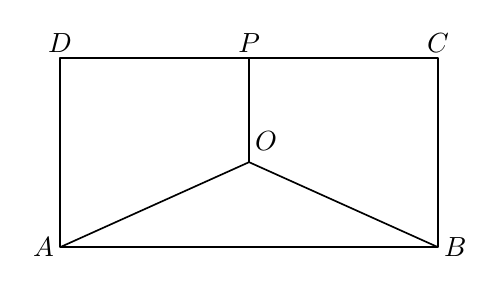
\begin{tikzpicture}[scale=1.2, line join=round]
    % 定义坐标 (按题意 AB=20, BC=10, 比例 2:1)
    \coordinate (A) at (0,0);
    \coordinate (B) at (4,0);
    \coordinate (C) at (4,2);
    \coordinate (D) at (0,2);
    \coordinate (P) at (2,2);
    % O点与A,B等距，故在AB的中垂线上，视觉上位置偏下
    \coordinate (O) at (2,0.9);

    % 绘制矩形边框
    \draw[semithick] (A) -- (B) -- (C) -- (D) -- cycle;
    
    % 绘制排污管道
    \draw[semithick] (A) -- (O) -- (B);
    \draw[semithick] (P) -- (O);

    % 标注字母
    \node[left, inner sep=2pt] at (A) {$A$};
    \node[right, inner sep=2pt] at (B) {$B$};
    \node[above, inner sep=2pt] at (C) {$C$};
    \node[above, inner sep=2pt] at (D) {$D$};
    \node[above, inner sep=2pt] at (P) {$P$};
    \node[above right, inner sep=2pt, yshift=2pt] at (O) {$O$};
\end{tikzpicture}